\section[Supplementary materials: pyRMSD]{Supplementary materials for: pyRMSD: a Python package for efficient pairwise RMSD matrix calculation and
handling}

Comparing the performance of different algorithms is not straightforward. We can deduce some theoretical bounds,
but these might be too general to have any practical value, especially when comparing similar algorithms. When this
happens, the only way to go is to compare implementations.

In our implementations, good code design (especially reusability) had a bigger priority than optimality. All three
algorithm implementations have been coded sharing the same framework, reusing as many pieces of code as possible. This
enhances the comparability of our implementations, which may be suboptimal in the same degree, giving us a unique
opportunity of making a more fair performance comparison between them.

All benchmark tests were performed in BSC's Minotauro \cite{barcelona_supercomputing_center_minotauro_2015}, which has been built with Intel Xeon E5649 CPUs and NVIDIA M2090
GPUs. Only 1 GPU was reserved for CUDA runs. OpenMP runs used six threads at most.

\subsection{Algorithm performance comparison}
In order to get a good overview of each algorithm{}'s performance, we have checked the time that each of the three
algorithms need to complete the execution of each one of pyRMSD's basic methods (oneVsFollowing, pairwiseMatrix and
iterativeSuperposition). A 30k trajectory of Ubiquitin (reading only \calpha atoms) was used. The oneVsFollowing method has
been tested without and with input coordinates rotation, as this last adds overhead to QCP implementation due to the
mandatory rotation matrix calculation (QCP does not need to calculate it otherwise).

For basic linear operations (see Fig.~\ref{fig:pyrmsd_supp:1}), QCP has the best performance of all three, even when the rotation matrix is
calculated (oneVsFollowing(r) and iterativeSuperposition). The use of OpenMP smooths differences so much that choosing
one algorithm over the other becomes a mere matter of preference (see Fig.~\ref{fig:pyrmsd_supp:2}).

\begin{figure}
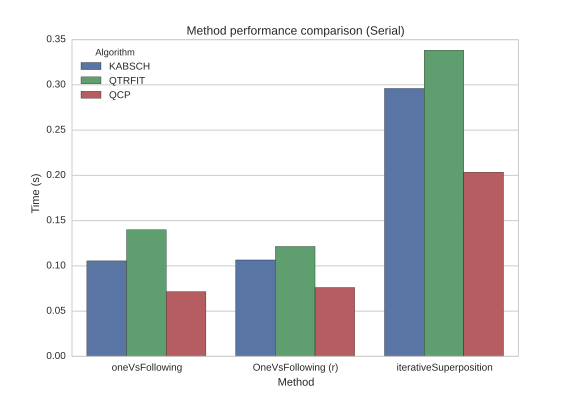
\includegraphics[width=\linewidth,height=\textheight,keepaspectratio]{pyrmsd_supp_serial_method_perf_comp.pdf}
\caption{ Comparison of the execution of three methods for the three available algorithm
implementations (serial).}
\label{fig:pyrmsd_supp:1}
\end{figure}

\begin{figure}
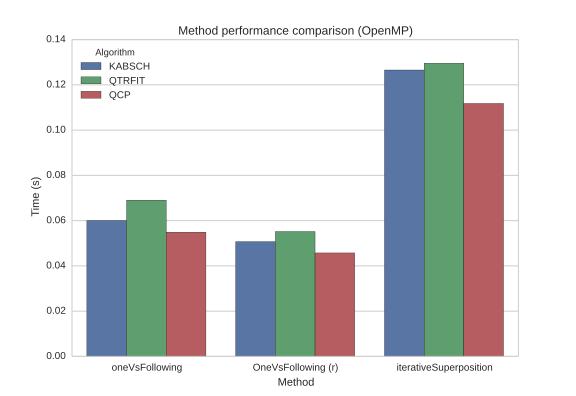
\includegraphics[width=\linewidth,height=\textheight,keepaspectratio]{pyrmsd_supp_openmp_method_perf_comp.pdf}
\caption{ Comparison of the execution of three methods for the three available algorithm
implementations (OpenMP).}
\label{fig:pyrmsd_supp:2}
\end{figure}

However, things change when comparing the performance of the pairwise matrix generation (see Fig.~\ref{fig:pyrmsd_supp:3}). Small performance
differences get amplified because of the quadratic nature of the problem. In this case, we observe that QCP excels by
achieving a 2x/4x speedup with respect to the other two, in both serial and OpenMP modes.

\begin{figure}
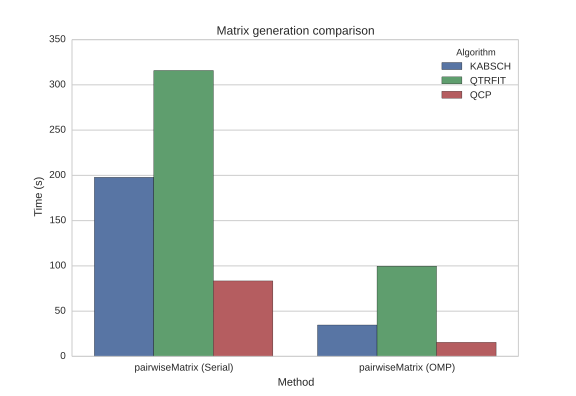
\includegraphics[width=\linewidth,height=\textheight,keepaspectratio]{pyrmsd_supp_matrix_gen_comp.pdf}
\caption{ Calculation time of a pairwise matrix from a 30k frames trajectory.} 
\label{fig:pyrmsd_supp:3}
\end{figure}

\subsection{QCP performance}
We want to compare all four implementations of QCP algorithm: serial, OpenMP, CUDA and CUDA with full matrix memory
allocation into the device. To this end, we will use the pairwiseMatrix method over Ubiquitin trajectories of 5, 10, 15,
20, 25, 30 and 35k frames.

We can see in the resulting plot (Fig.~\ref{fig:pyrmsd_supp:4}) that OpenMP version is about 5x faster than the serial one, and CUDA version
is about 8,5x faster.

\begin{figure}
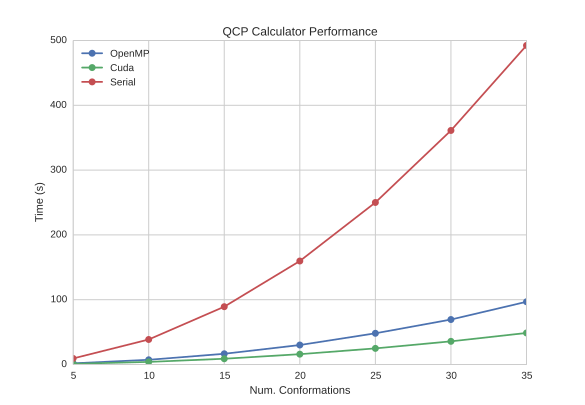
\includegraphics[width=\linewidth,height=\textheight,keepaspectratio]{pyrmsd_supp_qcp_perform_1.pdf}
\caption{ Performance comparison of serial, OpenMP and CUDA (single-precision) implementations of the QCP algorithm.}
\label{fig:pyrmsd_supp:4}
\end{figure}

After profiling the CUDA version, we saw that a considerable part of the time was spent in memory transactions from the
device to the host. The RMSD matrix is calculated line by line and, after each one of this calculations, the host
matrix representation is updated. This method can be successfully used in a broad range of GPUs, as it does not require
cards with big amounts of RAM. We implemented another method that holds the entire matrix in GPU's RAM. The speedup is
greater (11x compared with serial code), as memory transactions are performed only once (Fig.~\ref{fig:pyrmsd_supp:5}).

\begin{figure}
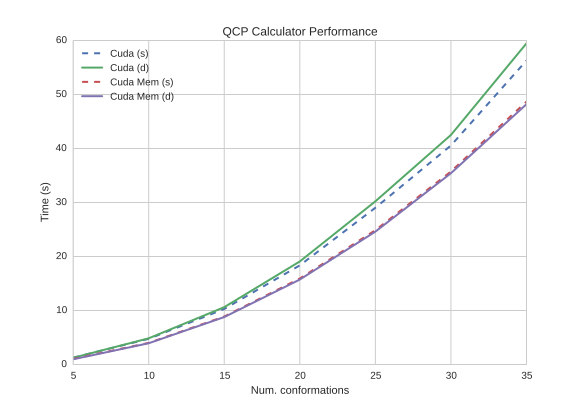
\includegraphics[width=\linewidth,height=\textheight,keepaspectratio]{pyrmsd_supp_qcp_perform_2.pdf}
\caption{ Performance comparison of CUDA implementations. 'Mem' versions hold the entire
matrix into memory, (s) versions use single-precision arrays and (d) versions use double-precision arrays.}
\label{fig:pyrmsd_supp:5}
\end{figure}

Finally, there are two things worth mentioning. The first one is that our CUDA implementation can be further improved by
enhancing work balance and memory coalescence. The second is that the use of single point precision in our QCP CUDA
implementation, contrary to what is expected, does not perform substantially better than the double precision
implementation. The reason for this behavior is again the big effort put into generalizing the code. pyRMSD uses
internally double-precision arrays to store coordinates and RMSD values. This implies that, when using GPUs without
double-precision support, a single-precision temporary buffer is to be filled at every host to device memory move.

\subsection{Input size response of \ QCP implementation}
The last benchmark established a clear relationship between the size of a trajectory (in frames) and the time needed to
do calculations. In this benchmark we want to fix the number of frames and test the impact of biomolecule sizes in
performance. The number of frames of the trajectory will be 10k, and the number of atoms of each one of the conformers
will be artificially increased at every step in order to calculate the pairwise RMSD matrix.

Both CUDA and OpenMP implementations, show a linear increase of the time needed to calculate the matrix (Fig.~\ref{fig:pyrmsd_supp:6}).
Incrementing conformer size does not increase or decrease performance.

\begin{figure}
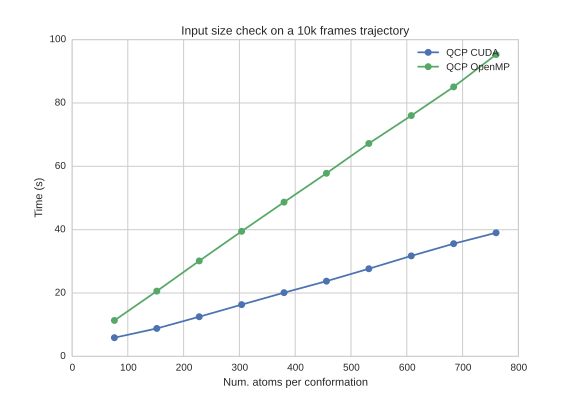
\includegraphics[width=\linewidth,height=\textheight,keepaspectratio]{pyrmsd_supp_input_size_check.pdf}
\caption{ Input size response of the OpenMP and CUDA versions of the QCP algorithm.}
\label{fig:pyrmsd_supp:6}
\end{figure}

\subsection{Accuracy check}
While KABSCH algorithm tries to find an optimal rotation matrix, QTRFIT and QCP will use quaternions in order to get
this rotation. Does the base method affect accuracy? In this test, we have applied the oneVsFollowing method over the
first frame of a 10k frames Ubiquitin trajectory. Then we have calculated the root mean square of the differences,
which will be our index of RMSD value variation. 

In Table \ref{tab:pyrmsd_supp:rmsd_accuracy}, we can see that all implementations have an RMS different than 0, which means that all algorithms have
calculated different RMSD values. Kabsch's algorithm and QTRFIT have close results in spite of their different
approaches to calculating the superposition. QCP CUDA single-precision floating point version differs the most, being the
double-precision version the most accurate of both.

\begin{table}
\centering
\begin{tabular}{ c c c c c c } 

\toprule
Method & KABSCH & QTRFIT & QCP & \specialcell{QCP CUDA\\(Single)} & \specialcell{QCP CUDA\\(Double)}\\
\midrule

KABSCH & ~ & 2.308e-12 & 2.678e-12 & 1.028e-03 & 2.689e-12\\
QTRFIT & ~ & ~ & 1.568e-12 & 1.028e-03 & 1.547e-12 \\
QCP & ~ & ~ & ~ & 1.028e-03 & 8.926e-13\\
\bottomrule

\end{tabular}
\caption{Root Mean Square of the RMSD array differences for each of the algorithms.}
\label{tab:pyrmsd_supp:rmsd_accuracy}
\end{table}

It is important to note that, although QCP solves the problems of prior methods like Diamond's \cite{diamond_note_1988} algorithm instability in
rotations close to 180�, it can suffer from convergence problems derived from the use of Newton-Raphson root-finding
method.

However, differences are generally small, and RMSD is often used qualitatively, which means that, unless we require high
precisions, all algorithm implementations are interchangeable.

\subsection{OpenMP scalability}
We want to study the scalability of the OpenMP version of each of the algorithms. To achieve it we have calculated the
pairwise RMSD matrix of a 30k frames trajectory of Ubiquitin, using a different number of threads for each execution
(from 1 to 6).

It is not difficult to see that we obtain a linear speedup, with a maximum of 5.6-5.8x for six threads (compared with the
one thread run), which is close to the theoretical maximum speedup (6x for six threads) (Fig.~\ref{fig:pyrmsd_supp:7}, \ref{fig:pyrmsd_supp:8}).

\begin{figure}
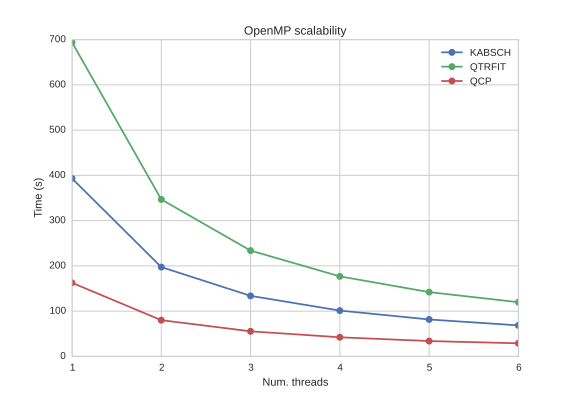
\includegraphics[width=\linewidth,height=\textheight,keepaspectratio]{pyrmsd_supp_omp_scalability.pdf}
\caption{ Time needed to compute a pairwise matrix from a 30k frames trajectory using a
different number of threads.}
\label{fig:pyrmsd_supp:7}
\end{figure}

\begin{figure}
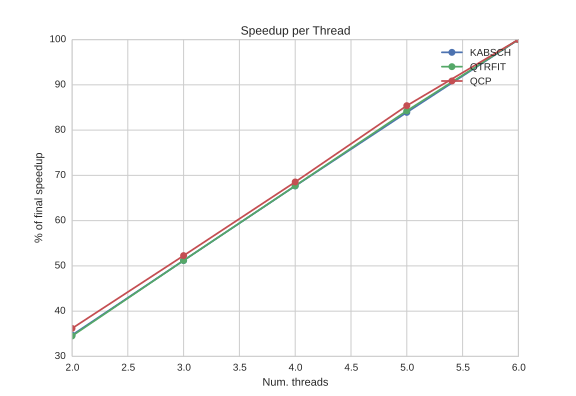
\includegraphics[width=\linewidth,height=\textheight,keepaspectratio]{pyrmsd_supp_speedup_per_thread.pdf}
\caption{ Percentage of speedup per thread added to the calculation. Speedup is almost
linear with number of threads.}
\label{fig:pyrmsd_supp:8}
\end{figure}

\subsection{Comparison with existing packages}
As a final test, we will compare pyRMSD with other software packages that include RMSD calculation features. We have
chosen four publicly available open source packages:

\begin{description}
	\item [g\_rms]  Is a C-written command line program part of the Gromacs \cite{berendsen_gromacs_1995} suite. Its main feature is the fast creation of
	distance matrices from trajectories.
	\item [Prody \cite{bakan_prody_2011-2}] A Python package which offers very interesting features to load and analyze biomolecule trajectories,
	including a complete PDB parser and a powerful selection language.
	\item [Biopython \cite{cock_biopython_2009-1}] A mature Python package which offers numerous bioinformatic computational tools.
	\item [PyVib2 \cite{fedorovsky_pyvib2_2007}] A pure Python package used to analyze vibrational motion and spectra of molecules.
\end{description}

Our comparison will be based on two measures: calculation time and integration complexity. To this aim we have created 4
scripts \footnote{The scripts can be found in \url{https://github.com/victor-gil-sepulveda/pyRMSD-Comparison.git}}. 
Every script calculates the RMSD
matrix of a trajectory twice, first using one of the aforementioned packages, and then replicating the same calculation
using pyRMSD (serial). Integration complexity has been measured as the ratio between the number of effective code lines
necessary to program the task with the tested package and pyRMSD. Performance has been calculated as the ratio of the time
needed to complete the task by the tested package over the time required by pyRMSD. All tests were performed on a workstation 
with an Intel Xeon W3530 CPU (four cores at 2.80GHz) with 12GB of RAM. 

\begin{sidewaystable}
\caption{Comparison of the time, lines of code, speedup and integration complexity (I.C.) needed to complete an RMSD collective operation.}
\centering
\begin{center}
\begin{tabular}{ r r c c c c c c }
\toprule
Method & Frames & Time (s) & Time pyRMSD(s)& 
 Lines of code & Lines of code (pyRMSD) & Speedup & I. C. \\ 
\midrule

\textbf{g\_rms} & 10 & 0.0564 & 0.0466 & 24 & 3 & 1.21 & 8 \\ 
~ & 100 & 0.7421 & 0.488 & ~ & ~ & 1.52 & ~ \\ 
~ & 1000 & 62.5245 & 14.6778 & ~ & ~ & 4.26 & ~ \\ 
\textbf{Prody} & 10 & 0.1698 & 0.0008 & 6 & 1 & 212.25 & 6 \\ 
~ & 100 & 3.408 & 0.0587 & ~ & ~ & 58.06 & ~ \\ 
~ & 1000 & 312.7806 & 6.0187 & ~ & ~ & 51.97 & ~ \\ 
\textbf{PyVib2} & 10 & 4.069 & 0.0001 & 7 & 1 & 40690.00 & 7 \\ 
~ & 100 & 450.1247 & 0.0995 & ~ & ~ & 4523.87 & ~ \\
~ & 1000 & 30332.6163 & 10.372 & ~ & ~ & 2924.47 & ~ \\ 
\textbf{Biopython} & 10 & 2.012 & 0.0008 & 8 & 1 & 2515.00 & 8 \\ 
~ & 100 & 219.6425 & 0.0572 & ~ & ~ & 3839.90 & ~ \\ 
~ & 1000 & 22003.5187 & 6.0966 & ~ & ~ & 3609.15 & ~ \\ 

\bottomrule
\end{tabular}
\end{center}
\label{tab:pyrmsd_supp:speedup}
\end{sidewaystable}

Table \ref{tab:pyrmsd_supp:speedup} shows that pyRMSD is always faster than the other packages. In the last three cases, this is because
that RMSD calculations are also written in pure python (which includes the use of numpy), while in pyRMSD these have
been written as C extensions. These packages have not been specifically designed to handle RMSD collective operations,
which explains why more lines of code are needed. Biopython and PyVib2 RMSD-related features are indeed constrained to
the pairwise RMSD case, while Prody can calculate rows of the matrix using only one function. This makes the last
faster and easier to use in this scenario. g\_rms is considerably faster than the others, as it has been written in C
and because of its narrower scope. However, to use it within a Python script, the user will need to create a wrapper to
control the program execution (here simplified by the utilization of the `expect' command), and a method to parse program
results. This adds extra complexity to the code as well as a performance penalty.






